\documentclass[dvipdfmx]{standalone}
\usepackage{tikz}
\usepackage[latin1]{inputenc}
\usetikzlibrary{shapes,arrows,shapes,shapes.geometric,calc}
\usetikzlibrary{positioning}


\begin{document}
\begin{tikzpicture}[scale=1]
    \tikzset{frame/.style={rectangle, draw, text width=7.8cm, text centered, minimum height=9.5cm, fill=white}};
\node (user) at (0cm, 6cm) {
\includegraphics[scale=0.15]{image/smart.png}};
\node (rap1) at (4cm, 6cm) {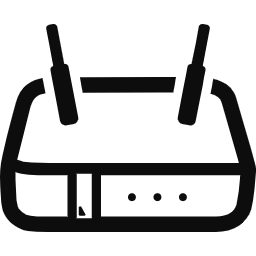
\includegraphics[scale=0.15]{image/lap.png}};
\node (rap2) at (7cm, 6cm) {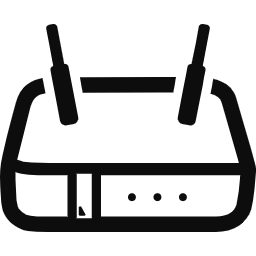
\includegraphics[scale=0.15]{image/lap.png}};
\node (lap) at (11cm, 6cm) {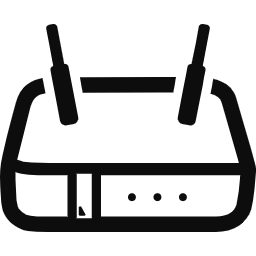
\includegraphics[scale=0.15]{image/lap.png}};
\node (gateway) at (15cm, 6cm) {
\includegraphics[scale=0.15]{image/gateway.png}};
\nade (pc) at (5.5cm,8cm) {
\includegraphics[scale=0.15]{image/pc.png}};
    %\node[frame](frame) at (3cm, 3cm){};


\end{tikzpicture}

\end{document}
 
